\setlength{\columnsep}{3pt}
\begin{flushleft}
	
	\paragraph{}
	\bigskip
	
	\begin{figure}[h!]
		\centering
		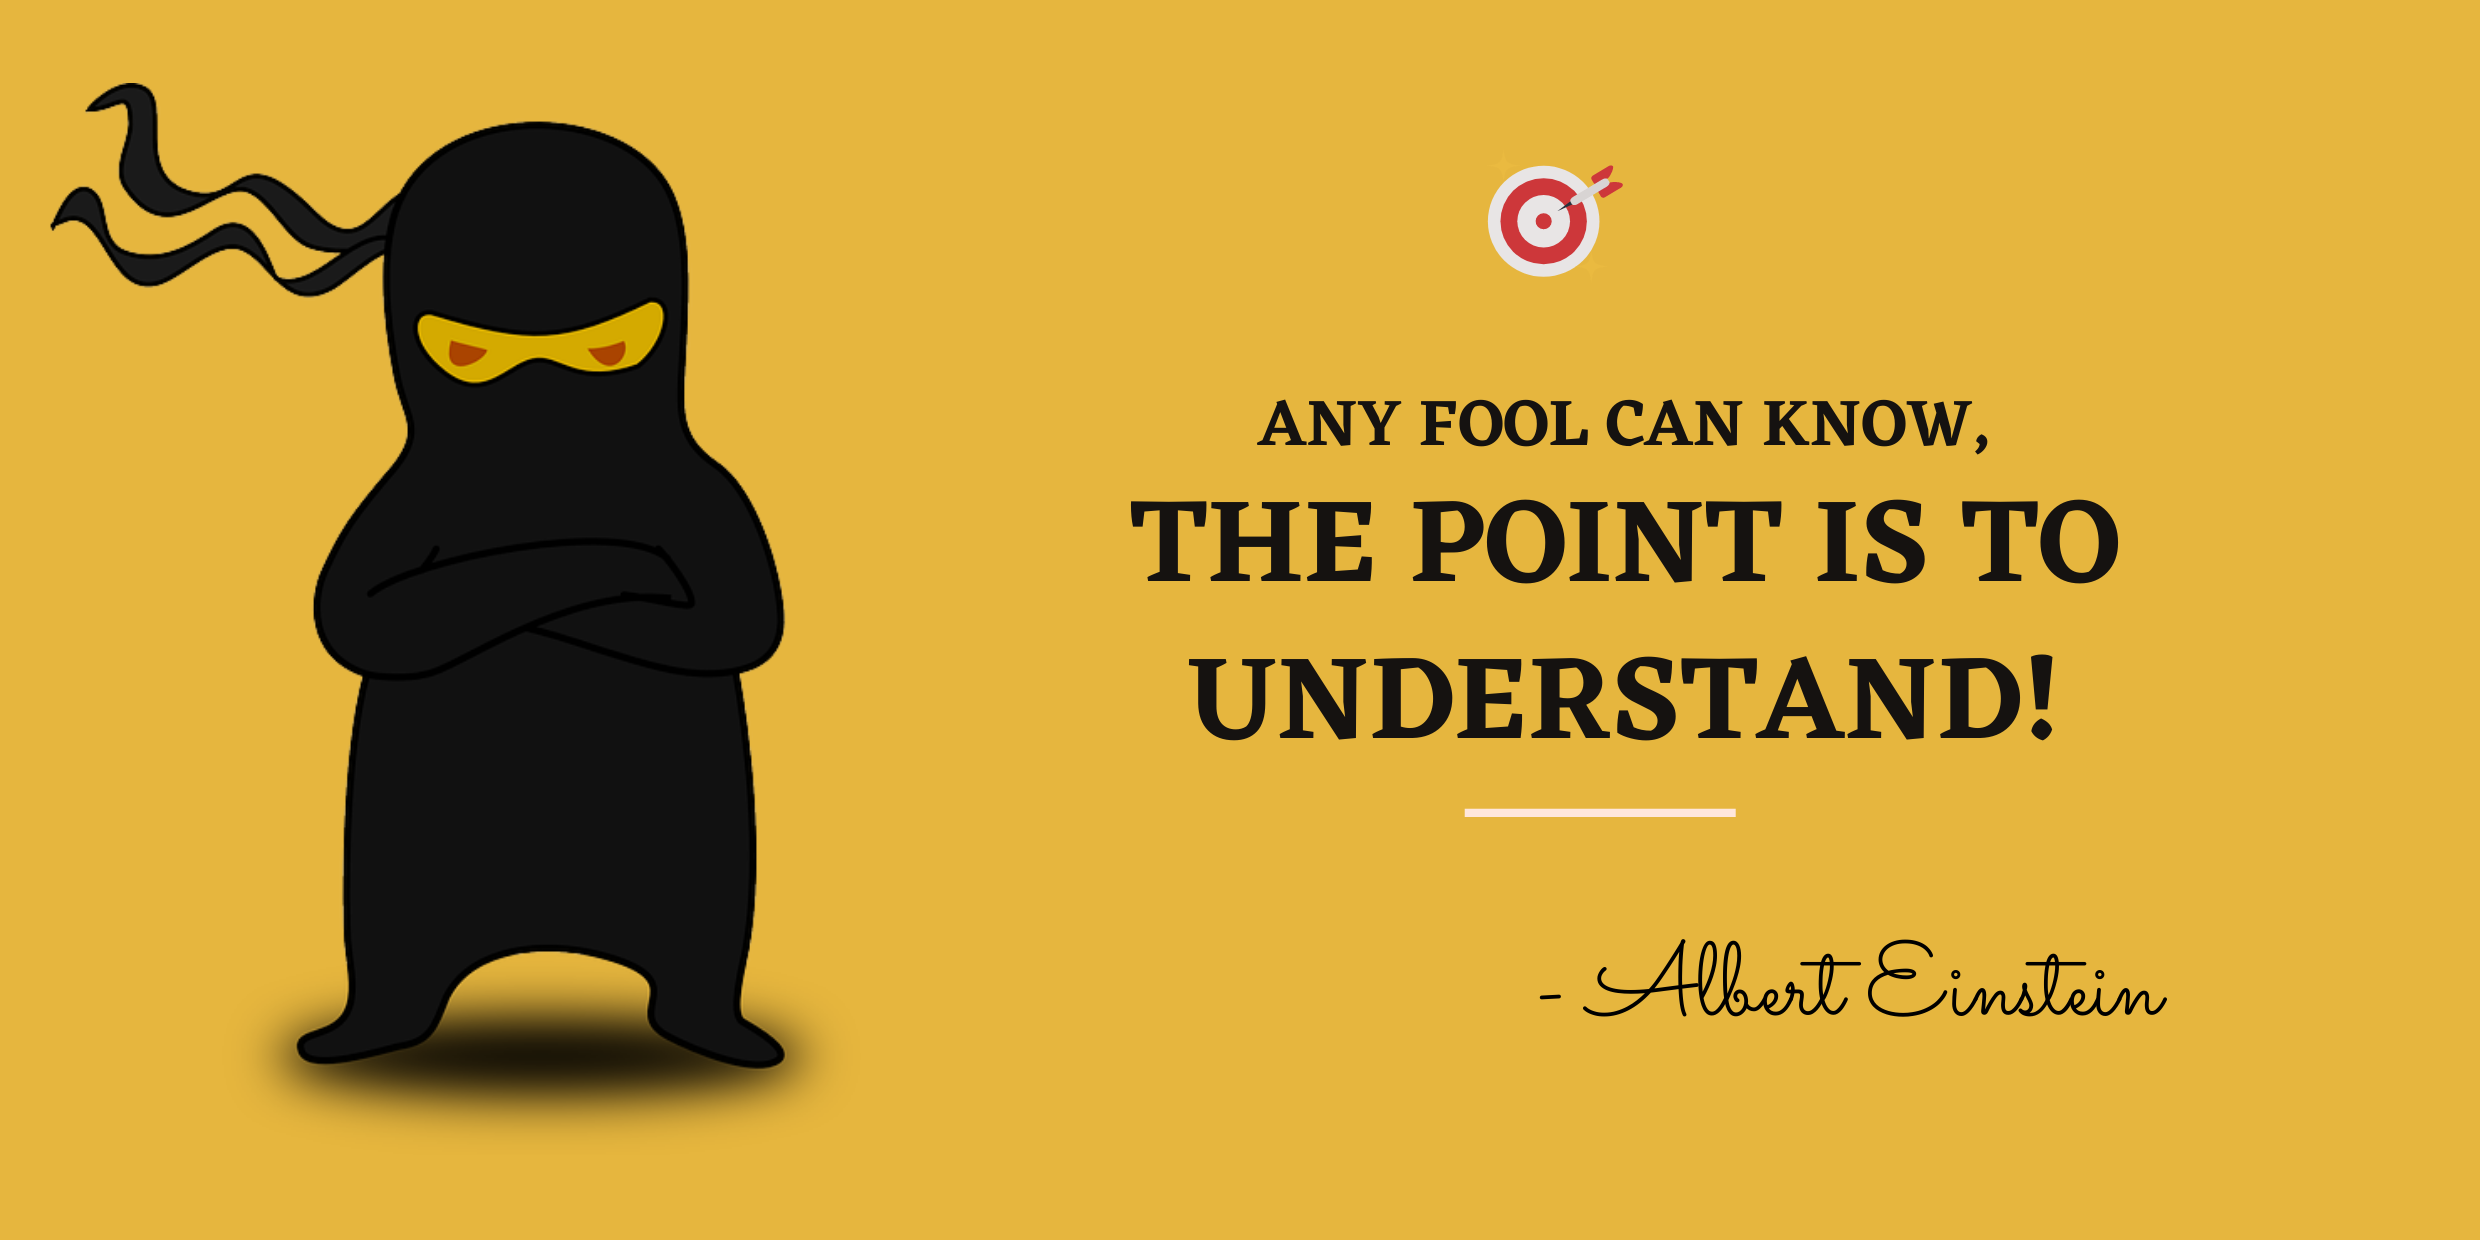
\includegraphics[scale=.2]{content/practise.jpg}
	\end{figure}	
	\begin{enumerate}
		
		\item \textbf{What is the full form of BIOS?}
		\begin{enumerate}[label=(\alph*)]
			\item Basic Input Output System    %correct
			\item Begin Input Output System
			\item Basic Intake Outtake System
			\item Basic Input Output State
		\end{enumerate}
		\bigskip
		\bigskip	

		\item \textbf{What is the full form of GRUB?}
		\begin{enumerate}[label=(\alph*)]
			\item GRand Unified Bootleader    
			\item GRand Unified Bootloader   %correct
			\item GRand Union Bootloader
			\item GRand Union Bootleader
		\end{enumerate}
		\bigskip
		\bigskip	
		
		\item \textbf{What is the full form of POST?		}	
		\begin{enumerate}[label=(\alph*)]
			\item Power On Self Terminator
			\item Power On System Test    
			\item Pity On Self Test    
			\item Power On Self Test    %correct
		\end{enumerate}
		\bigskip
		\bigskip	
		\newpage
		\item \textbf{What is the full form of MBR?}
		\begin{enumerate}[label=(\alph*)]
			\item Mini Boot Recorder
			\item Mini Boot Reader
			\item Mini Booting Recorder   
			\item Master Boot Recorder    %correct
		\end{enumerate}
		\bigskip
		\bigskip	
		
		\item \textbf{What is the size of MBR?}
		\begin{enumerate}[label=(\alph*)]
			\item 512 bytes   %correct
			\item 528 bytes  
			\item 446 bytes 
			\item 518 bytes   
		\end{enumerate}
		\bigskip
		\bigskip	

		\item \textbf{What is the size of partition table in MBR?}
		\begin{enumerate}[label=(\alph*)]
			\item 512 bytes
			\item 412 bytes   
			\item 64 bytes     %correct
			\item 446 bytes   
		\end{enumerate}
		\bigskip
		\bigskip	

		\item \textbf{What is a magic number?}
		\begin{enumerate}[label=(\alph*)]
			\item Final 2 bytes in MBR that contains the boot signature    
			\item Final 12 bytes in MBR that contain boot signature    
			\item Final 64 bytes in MBR that contains boot signature    
			\item Final 446 bytes in MBR that contains boot signature    %correct
		\end{enumerate}
		\bigskip
		\bigskip	

		\item \textbf{What is the location of grub2 bootloader?}
		\begin{enumerate}[label=(\alph*)]
			\item /etc/boot/grub2/grub.cfg
			\item /boot/grub.cfg
			\item /boot/grub2/grub.cfg  %correct
			\item /grub2/grub.cfg
		\end{enumerate}
		\bigskip
		\bigskip
		\newpage
		\item \textbf{Who loads the /boot/initramfs-xxxxx.img file?}
		\begin{enumerate}[label=(\alph*)]
			\item Linux modules
			\item Linux kernel   %correct
			\item Linux bootloader grub2  
			\item linuxrc
		\end{enumerate}
		\bigskip
		\bigskip	

		\item \textbf{Which is the first process initiated by the Linux kernel?}
		\begin{enumerate}[label=(\alph*)]
			\item systemd  %correct
			\item graphical.target
			\item initramfs
			\item initrd
		\end{enumerate}
		\bigskip
		\bigskip

		\item \textbf{Which directory stores all target unit files in RHEL? (Select all that applies.)}
		\begin{enumerate}[label=(\alph*)]
			\item /usr/lib/systemd/system/  %correct
			\item /etc/systemd/system/  %correct
			\item /usr/share/lib/systemd/system
			\item /usr/lib/system
		\end{enumerate}
		\bigskip
		\bigskip

		\item \textbf{Which of the following command is used to switch to multi-user.target in Linux?}
		\begin{enumerate}[label=(\alph*)]
			\item init 5 
			\item init 6 
			\item init 3  %correct  
			\item init 0 
		\end{enumerate}
		\bigskip
		\bigskip

		\item \textbf{Which of the following command is used to poweroff server in Linux?}
		\begin{enumerate}[label=(\alph*)]
			\item init 5 
			\item init 6 
			\item init 3 
			\item init 0  %correct  
		\end{enumerate}
		\bigskip
		\bigskip

		\item \textbf{Which of the following command is used to switch to graphical.target in Linux?}
		\begin{enumerate}[label=(\alph*)]
			\item init 5   %correct
			\item init 6 
			\item init 3 
			\item init 0   
		\end{enumerate}
		\bigskip
		\bigskip

		\item \textbf{Which of the following command is used to reboot server in Linux?}
		\begin{enumerate}[label=(\alph*)]
			\item init 5  
			\item init 6   %correct
			\item init 3 
			\item init 0   
		\end{enumerate}
		\bigskip
		\bigskip

		\item \textbf{Which of the following command is used to set the default runlevel/target in Linux?}
		\begin{enumerate}[label=(\alph*)]
			\item systemctl setdefault  target-name
			\item systemctl set-default  target-name  %correct
			\item systemctl set target-name
			\item systemctl set default target-name
		\end{enumerate}
		\bigskip
		\bigskip
		
	\end{enumerate}
\end{flushleft}
